\documentclass{article}
\usepackage[a4paper,margin=2cm]{geometry}
\usepackage[colorlinks=true, linkcolor=blue, urlcolor=blue]{hyperref}
\usepackage{multirow,amsmath,listings,xcolor,graphicx,tikz}
\usetikzlibrary{shapes,positioning,shadows,matrix}

\definecolor{codegreen}{rgb}{0,0.6,0}
\definecolor{codegray}{rgb}{0.5,0.5,0.5}
\definecolor{codepurple}{rgb}{0.58,0,0.82}
\definecolor{backcolour}{rgb}{0.95,0.95,0.92}

% Define Python style
\lstdefinestyle{mystyle}{
    backgroundcolor=\color{backcolour},   
    commentstyle=\color{codegreen},
    keywordstyle=\color{magenta},
    numberstyle=\tiny\color{codegray},
    stringstyle=\color{codepurple},
    basicstyle=\ttfamily\footnotesize,
    breakatwhitespace=false,         
    breaklines=true,                 
    captionpos=b,                    
    keepspaces=true,                 
    numbers=left,                    
    numbersep=5pt,                  
    showspaces=false,                
    showstringspaces=false,
    showtabs=false,                  
    tabsize=2
}

\definecolor{titlepagecolor}{cmyk}{1,.60,0,.40}
\DeclareFixedFont{\titlefont}{T1}{ppl}{b}{it}{0.5in}

% The following code is borrowed from: https://tex.stackexchange.com/a/86310/10898

\newcommand\titlepagedecoration{%
\begin{tikzpicture}[remember picture,overlay,shorten >= -10pt]

\coordinate (aux1) at ([yshift=-15pt]current page.north east);
\coordinate (aux2) at ([yshift=-410pt]current page.north east);
\coordinate (aux3) at ([xshift=-4.5cm]current page.north east);
\coordinate (aux4) at ([yshift=-150pt]current page.north east);

\begin{scope}[titlepagecolor!40,line width=12pt,rounded corners=12pt]
\draw
  (aux1) -- coordinate (a)
  ++(225:5) --
  ++(-45:5.1) coordinate (b);
\draw[shorten <= -10pt]
  (aux3) --
  (a) --
  (aux1);
\draw[opacity=0.6,titlepagecolor,shorten <= -10pt]
  (b) --
  ++(225:2.2) --
  ++(-45:2.2);
\end{scope}
\draw[titlepagecolor,line width=8pt,rounded corners=8pt,shorten <= -10pt]
  (aux4) --
  ++(225:0.8) --
  ++(-45:0.8);
\begin{scope}[titlepagecolor!70,line width=6pt,rounded corners=8pt]
\draw[shorten <= -10pt]
  (aux2) --
  ++(225:3) coordinate[pos=0.45] (c) --
  ++(-45:3.1);
\draw
  (aux2) --
  (c) --
  ++(135:2.5) --
  ++(45:2.5) --
  ++(-45:2.5) coordinate[pos=0.3] (d);   
\draw 
  (d) -- +(45:1);
\end{scope}
\end{tikzpicture}%
}
\usepackage{tcolorbox}
\tcbuselibrary{skins}
\usepackage{psvectorian}
\renewcommand*{\psvectorianDefaultColor}{white}%

\tcbset{
    Baystyle/.style={
        sharp corners,
        boxrule=3pt,
        colback=white,
        height=\textheight,
        width=\textwidth,
        borderline={8pt}{-11pt}{},
    }
}

% Set Python style
\lstset{style=mystyle}

\begin{document}
    \begin{titlepage} % Suppresses headers and footers on the title page
    \begin{tcolorbox}[Baystyle]{
        \centering % Centre everything on the title page
        \vspace*{4\baselineskip}
        \includegraphics[scale=0.15]{Images/BUET_LOGO.png}
	
	\scshape % Use small caps for all text on the title page
	
	\vspace*{3\baselineskip} % White space at the top of the page
	
	\rule{0.75\textwidth}{1.6pt}\vspace*{-\baselineskip}\vspace*{2pt} % Thick horizontal rule
	\rule{0.75\textwidth}{0.4pt} % Thin horizontal rule
	
	\vspace*{0.75\baselineskip} % Whitespace above the title
	
	{\LARGE A REPORT\\ ON\\ B+ TREE\\} % Title
	
	\vspace{0.75\baselineskip} % Whitespace below the title
	
	\rule{0.75\textwidth}{0.4pt}\vspace*{-\baselineskip}\vspace{3.2pt} % Thin horizontal rule
	\rule{0.75\textwidth}{1.6pt} % Thick horizontal rule
	
	\vspace{2\baselineskip} % Whitespace after the title block
	CSE300: Technical Writing and Presentation\\ % Subtitle or further description
	\vspace*{5\baselineskip} % 	
	Prepared By
	
	\vspace{0.5\baselineskip} % Whitespace before the editors
	{\scshape\Large Anup Halder Joy - 2005005 \\ Afzal Hossan - 2005021 \\ Asif Karim - 2005024 \\} % Editor list
	
	\vspace{0.5\baselineskip} % Whitespace below the editor list
 {\scshape Computer Science and Engineering \\ Bangladesh University of Engineering and Technology\\} % Editor affiliation
        \vspace*{10\baselineskip}
 }
\end{tcolorbox}
\end{titlepage}
    \newgeometry{left=3cm,right=5cm,top=3cm,bottom=3cm}
    \tableofcontents
    \vspace*{3\baselineskip}
    \listoffigures
    \vspace*{3\baselineskip}
    \listoftables
    \titlepagedecoration
    \restoregeometry
    \newpage
    \section{Definition}
    \begin{itemize}
        \item A B+ tree is an m-ary tree with a large number of children per node. A B+ tree consists of a root, internal nodes and leaves. The root may be either a leaf or a node with two or more children.\cite{navathe2010fundamentals}
        \item  A B+ Tree is a \textcolor{red}{self-balancing} tree data structure that maintains sorted data and allows searches, sequential access, insertions, and deletions
        \item The primary value of a B+ tree is in storing data for efficient retrieval in a block-oriented storage context — in particular, filesystems. This is primarily because unlike binary search trees, B+ trees have very high fanout (number of pointers to child nodes in a node, typically on the order of 100 or more), which reduces the number of I/O operations required to find an element in the tree.
    \end{itemize}
    
    \section{History}
    \begin{itemize}
        \item The history of B+ trees dates back to their invention by Rudolf Bayer and Edward M. McCreight in 1972. The B+ tree was introduced as an improvement over the original B-tree data structure, which was also developed by Bayer and McCreight in 1970. Bayer and McCreight never explained what, if anything, the B stands for; Boeing, balanced, between, broad, bushy, and Bayer have been suggested. McCreight has said that "the more you think about what the B in B-trees means, the better you understand B-trees".
        \begin{figure}[ht]
            \centering
            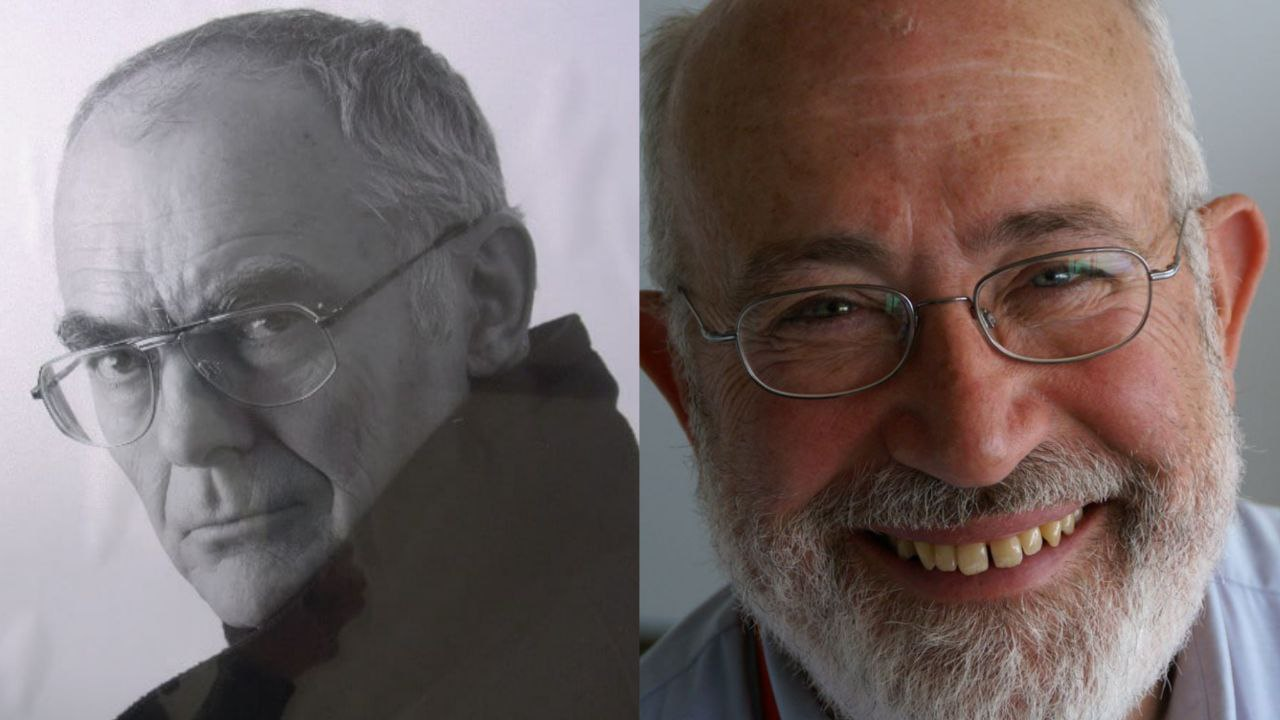
\includegraphics[scale=0.2]{Images/image.png}\\
            \hspace{20pt}Rudolf Bayer\hspace{60pt}Edward M. McCreight \end{figure}
        \item The B+ tree was designed to address certain limitations of the B-tree, particularly in the context of file systems and database management systems. The key innovation of the B+ tree lies in the way it organizes and stores data.
    \end{itemize}
    \section{Evolution of B+ Tree}
    \tikzstyle{block} = [rectangle, draw, top color=blue!30, bottom color=blue!5, text width=8em, text centered, rounded corners, minimum height=3em]
    \tikzstyle{line} = [draw, -latex] 
    \begin{figure}[ht]
        \centering
        \begin{tikzpicture}[very thick,node distance=1.75cm, every node/.style={drop shadow}]
                % Nodes
                \node [block, fill=yellow] (bst) {Binary Search Tree};
                \node [block, below of=bst, fill=yellow] (mWaytree) {M-way Search Tree};
                \node [block, below of=mWaytree, fill=yellow] (btree) {B Tree};
                \node [block, below of=btree, fill=yellow] (bplustree) {B+ Tree};
            
                % Arrows
                {\path [line] (bst) -- (mWaytree);}
                {\path [line] (mWaytree) -- (btree);}
                {\path [line] (btree) -- (bplustree);}
            \end{tikzpicture}
        \caption{Evolution of B+ Tree}
    \end{figure}

    \subsection*{}     The evolution of the B+ tree from its predecessors marks a significant advancement in data structure design, particularly in the realm of database management systems.
    \begin{itemize}
        \item \textbf{Binary Search Tree:} Beginning with the Binary Search Tree (BST), which provided efficient searching but suffered from unbalanced structures leading to suboptimal performance in certain scenarios, such as highly skewed or sorted data distributions.
        \subsection*{}
        \usetikzlibrary{arrows,positioning, calc}
        \tikzstyle{vertex}=[draw,top color =blue!30,bottom color = blue!5,circle,minimum size=0.60cm,inner sep=0pt]
        \begin{figure}[ht]
            \centering
            \begin{tikzpicture}[very thick,level/.style={sibling distance=70mm/#1},every node/.style={drop shadow}]
            \node [vertex] (r){$17$}
            child {
                node [vertex] (a) {$9$}
                child {
                    node [vertex] {$3$}
                    child {
                        node [vertex] {$-3$}
                    }
                    child {
                         node [vertex] {$8$}
                    }
                }
                child {
                    node [vertex] {$11$}
                    child {
                        node [vertex] {$15$}
                    }
                    child {
                        node [vertex](l1) {$17$}
                    }
                }
            }
            child {
                node [vertex] {$19$}
                child {
                    node [vertex] {$18$}
                }
                child {
                    node [vertex](l2) {$20$}
                }
            };
            \end{tikzpicture}
            \caption{Binary Search Tree}
        \end{figure}
                
        \item \textbf{M-way Tree:} The m-way tree addressed this imbalance by allowing multiple keys per node, improving balance and thus mitigating some of the inefficiencies of BSTs. However, it still faced \textcolor{red}{limitations in disk-based storage systems}, where frequent disk accesses could hamper performance.
        \subsection*{}
        \begin{figure}[ht]
            \centering          
            \tikzset{ every matrix/.style={inner sep=-\pgflinewidth,matrix of math nodes,
            column sep=-\pgflinewidth,
            nodes={ draw,top color =blue!30,bottom color = blue!5, minimum size=.60cm, anchor=center,fill=brown!20
            }
            }
            }

            \begin{tikzpicture}[very thick,every node/.style={drop shadow}]
            \matrix[above] (t1) at (0,0) {18 & 44 & 76 & 198\\};
            \matrix[below] (b1) at (0,0) {\bullet & \times & \times & \bullet & \bullet\\};
            \matrix[above] (t21) at (-3.5,-2.5) {7 & 12\\};
            \matrix[below] (b21) at (-3.5,-2.5) {\times & \bullet & \times\\};
            \matrix[above] (t22) at (0,-2.5) {80 & 92 & 141\\};
            \matrix[below] (b22) at (0,-2.5) {\bullet & \times & \times & \bullet\\};
            \matrix[above] (t23) at (3.5,-2.5) {262\\};
            \matrix[below] (b23) at (3.5,-2.5) {\times & \times\\};
            \matrix[above] (t31) at (-6.5,-5.5) {8 & 10\\};
            \matrix[below] (b31) at (-6.5,-5.5) {\times & \times & \times\\};
            \matrix[above] (t32) at (-2.5,-5.5) {77\\};
            \matrix[below] (b32) at (-2.5,-5.5) {\times & \times\\};
            \matrix[above] (t33) at (2.5,-5.5) {148 & 151 & 172 & 186\\};
            \matrix[below] (b33) at (2.5,-5.5) {\times & \times & \times & \times &             \times\\};
            \draw[black] (b1-1-1.center) -- (t21-1-1.north east)
                (b1-1-4.center) -- (t22-1-3.north)
                (b1-1-5.center) -- (t23-1-1.north west)
                (b21-1-2.center) -- (t31-1-1.north east)
                (b22-1-1.center) -- (t32-1-1.north)
                (b22-1-4.center) -- (t33-1-2.north east);             
            \end{tikzpicture}
            \caption{m-way Tree (m =5)}
        \end{figure}
        \pagebreak
        \item \textbf{B Tree:} The B tree sought to remedy this by optimizing for external storage, but its design \textcolor{red}{lacked efficient support for range queries and sequential access} due to its internal structure, leading to suboptimal performance in certain database operations.
        \subsection*{}
        
        \begin{figure}[ht]
            \centering
            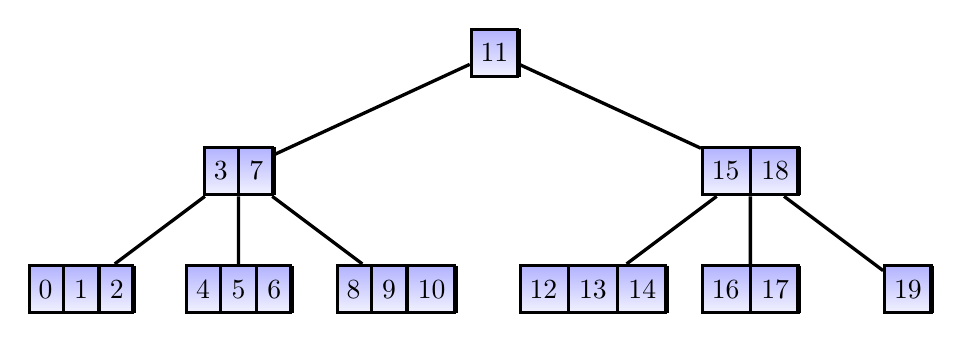
\begin{tikzpicture}[very thick,every node/.style={drop shadow}]
            \tikzstyle{bplus}=[draw,top color=blue!30,bottom color=blue!5,minimum size=.60cm,rectangle split, rectangle split horizontal,rectangle split ignore empty parts,draw, fill=brown!20]
            \tikzstyle{every node}=[bplus]
            \tikzstyle{level 1}=[sibling distance=65mm]
            \tikzstyle{level 2}=[sibling distance=20mm]

            \node {11} [-]
                 child {node {3 \nodepart{two} 7}
                    child {node {0 \nodepart{two} 1 \nodepart{three} 2}}
                    child {node {4 \nodepart{two} 5 \nodepart{three} 6}}
                    child {node {8 \nodepart{two} 9 \nodepart{three} 10}}
                }
                child {node {15 \nodepart{two} 18}
                    child[sibling distance=20mm] {node {12 \nodepart{two} 13 \nodepart{three} 14}}
                    child {node {16 \nodepart{two} 17}}
                    child {node {19}}
                };
            \end{tikzpicture}
            \caption{B Tree}
        \end{figure}
        
        \item \textbf{B+ Tree:} Building upon all these challenges, the B+ tree refined this concept by separating internal nodes from leaf nodes, enhancing sequential access and range queries through its leaf-level linked lists while maintaining the balanced properties of its predecessors. This progression reflects a continual refinement in addressing the challenges of storage and retrieval in database systems, culminating in the robust and widely adopted B+ tree data structure.
        \subsection*{}
        
        \begin{figure}
            \centering
            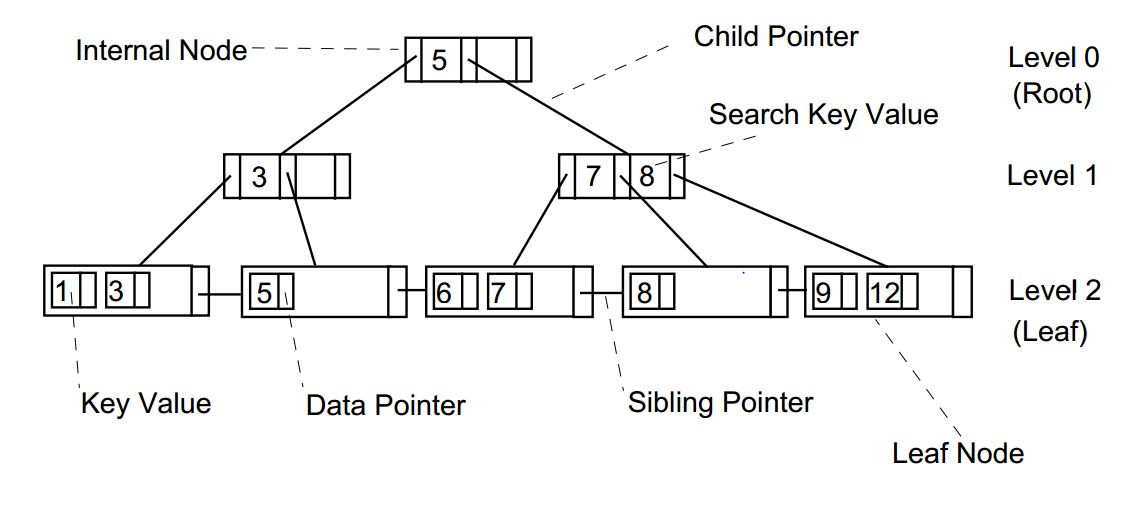
\includegraphics[scale=0.5]{Images/B+tree.jpg}
            \caption{B+ Tree}
        \end{figure}
        
    \end{itemize}
    \section{Nodes of B+ Tree}
    \subsection{Internal Node Structure}
    The structure of an internal node in a B+ tree is as follows:

    \begin{itemize}
        \item Sorted keys: Contains sorted keys that guide the search process.
        \item Child Pointers: Pointers to child nodes for navigating the tree.
        \item Variable Size: Can accommodate a variable number of keys and child pointers.
        \item Balance: Techniques like splitting and merging ensure balanced tree structure.
    \end{itemize}
    \begin{figure}[ht]
        \centering
        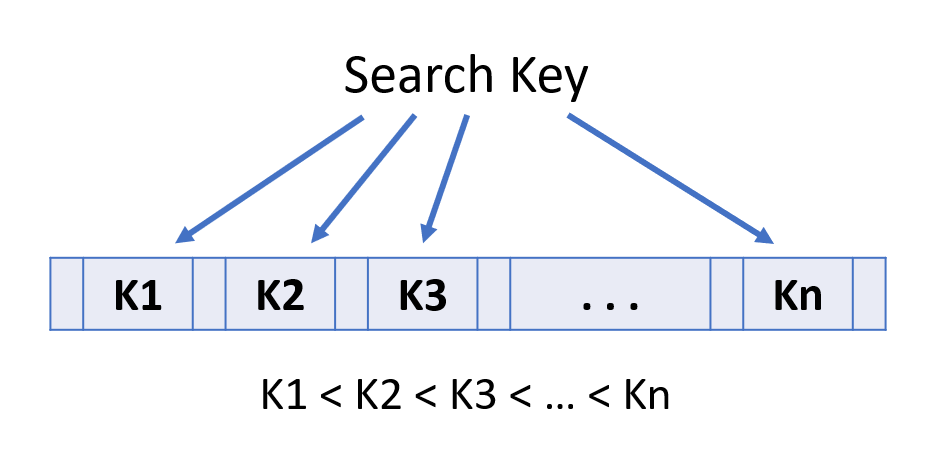
\includegraphics[scale = 0.4]{Images/InternalNode.png}
        \caption{Internal Node Structure}
    \end{figure}
    \subsection{Leaf Node Structure}
    The structure of a leaf node in a B+ tree is simple:

    \begin{itemize}
        \item Sorted Entries: Contains sorted keys and pointers to actual data entries.
        \item Data Entries: Stores actual data associated with the keys.
        \item Pointer to Next Leaf: Often linked to the next leaf node for     efficient sequential access.
        \item Variable Size: Entries can be of fixed or variable size.
        \item Occupancy Management: Techniques like splitting and merging maintain optimal balance.
    \end{itemize}
    \begin{figure}[ht]
        \centering
        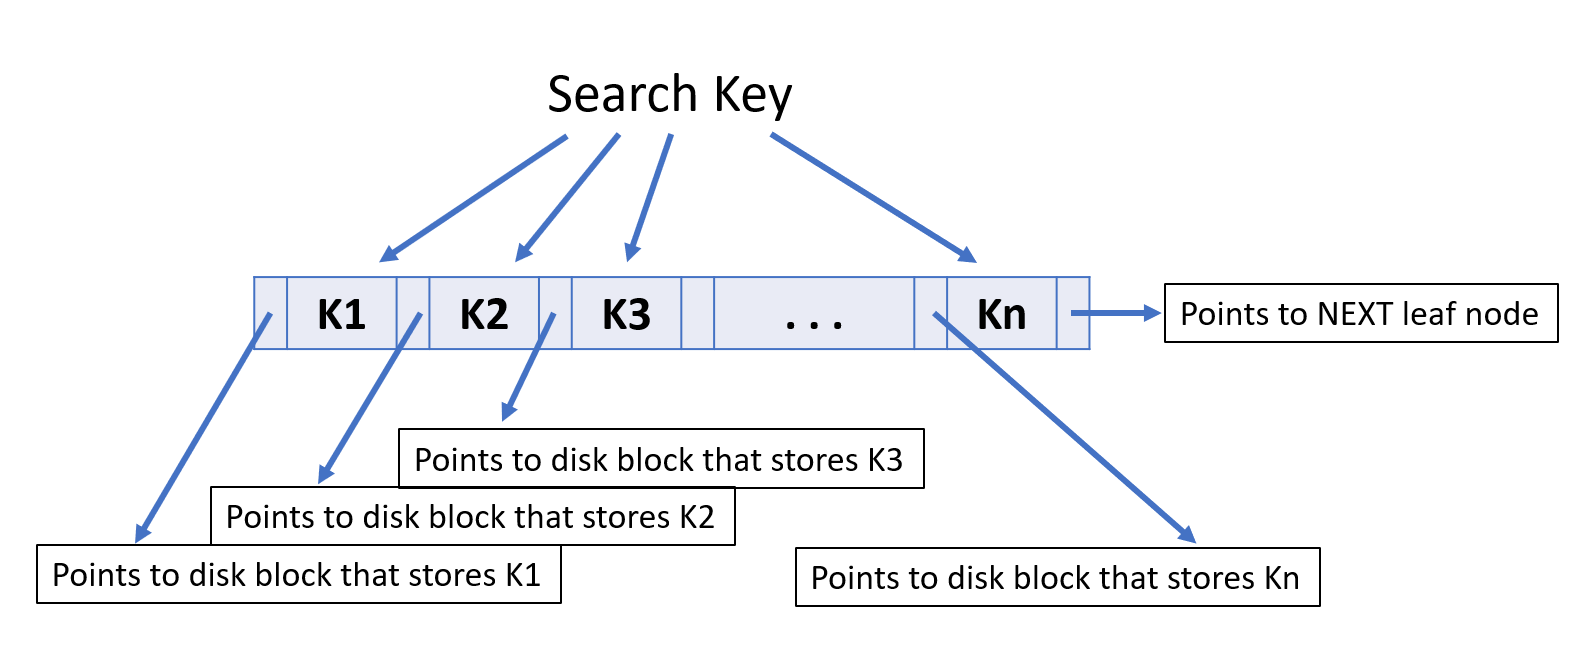
\includegraphics[scale = 0.35]{Images/LeafNode.png}
        \caption{Leaf Node Structure}
    \end{figure}
    Visit \href{https://www.cs.emory.edu/~cheung/Courses/554/Syllabus/3-index/B-tree=intro3.html}{here} to learn more.
    \subsection{Node Bounds}
Node bounds are crucial in B+ trees, ensuring balanced structure, efficient search, and optimal space utilization. By setting limits on the maximum number of keys and children a node can hold, these bounds prevent nodes from becoming excessively large or sparse. This balance enhances search efficiency by streamlining the traversal and narrowing down the search space.
\vspace{12pt}

In addition, node bounds significantly contribute to the efficiency of search operations within the tree. By limiting the number of keys stored in each node, the search process is simplified. With fewer keys to examine during traversal, search algorithms can quickly narrow down the search space and locate the desired data, leading to faster query response times.
\vspace{12pt}

Furthermore, node bounds provide clear guidelines for node splitting and merging procedures, essential for maintaining the tree's balance after insertions and deletions. When a node exceeds its maximum capacity, it must be split into two nodes, each adhering to the defined bounds. Similarly, if a node becomes too sparsely populated, it may need to be merged with its neighboring nodes to optimize space utilization.
\vspace{12pt}

In addition to preserving balance and facilitating operations, node bounds also contribute to space efficiency within the tree. By controlling the maximum number of keys and children per node, B+ trees can effectively utilize available memory resources without excessive waste or fragmentation. This efficient space management is particularly important in scenarios with limited memory or disk storage capacity.
\vspace{12pt}

Overall, node bounds are indispensable in B+ trees, playing a pivotal role in maintaining balance, optimizing search efficiency, guiding tree operations, and maximizing space utilization. Their careful definition and adherence are essential for the effective organization and performance of B+ tree-based data structures.

\begin{table}[ht]
\centering
\begin{tabular}{| c | c | c | c | c |}
    \hline
      \textbf{Node} & \textbf{Min} & \textbf{Max} & \textbf{Min} & \textbf{Max}\\
      \textbf{Type} &\textbf{\#Keys}&\textbf{\#Keys}& \textbf{\#Child}&\textbf{\#Child}\\
      \hline
      Root & \multirow{2}{*}{1}&\multirow{2}{*}{$M-1$}&\multirow{2}{*}{2\cite{navathe2010fundamentals}}&\multirow{2}{*}{M}\\
      Node & & & & \\
      \hline
       Internal& \multirow{2}{*}{$\lceil{\frac{M}{2}}\rceil - 1$ }&\multirow{2}{*}{$M-1$} &  \multirow{2}{*}{$\lceil{\frac{M}{2}}\rceil $ } & \multirow{2}{*}{M}\\
       Node& & & & \\
     \hline
     Leaf & \multirow{2}{*}{$\lceil{\frac{M}{2}}\rceil - 1 $ }&\multirow{2}{*}{$M-1$} & \multirow{2}{*}{0} & \multirow{2}{*}{0}\\
       Node& & & & \\
     \hline
\end{tabular}\\
M = Order of B+ Tree
\caption{Node bounds}
\end{table}

\section{Operations on B+ Tree}
    \subsection{Insertion }
        Before adding an item to a B + tree, it is crucial to consider the following criteria: \begin{enumerate}
            \item The root node must have a minimum of two children.
            \item Each node, excluding the root, can accommodate up to a maximum         of $m$ children and at least $\frac{m}{2}$ children.
            \item Each node can hold a maximum of $m - 1$ keys and a minimum of $\lceil\frac{m}{2}\rceil - 1$ keys.
        \end{enumerate}
        \vspace{12pt}
        The insertion process follows these steps:
        \begin{enumerate}
            \item Locate the appropriate leaf node for insertion since every element is inserted into a leaf node.
            \item Insert the key into the leaf node.
           
           \begin{itemize}
               \item \textbf{Case I:}\\
                 If the leaf node isn't at full capacity, insert the key in increasing order.
           
               \item \textbf{Case II:}
                 \begin{enumerate}
                    \item If the leaf node reaches its full capacity, insert the key in  increasing order and balance the tree by following these steps:
                    \item Split the node at the $\frac{m}{2}$th position.
                    \item Add the $\lceil \frac{m}{2} \rceil$th key to the parent node.
                    \item If the parent node is also full, repeat steps (b) to (c).
                 \end{enumerate}
           \end{itemize}
        \end{enumerate}
        \vspace{12pt}
        Let's see and example of insertion in order m = 3 B+ tree. The elements to be inserted are 5,15, 25, 35, 45.
        \vspace{12pt}
        \begin{center}
              \color{red}\textbf{Insert 5}   
        \end{center}
        \begin{figure}[ht]
            \centering
            
\includegraphics[scale=0.8]{Images/bi1.jpg}
        \end{figure}
        \pagebreak
        \begin{center}
              \color{red}\textbf{Insert 15}   
        \end{center}
        \begin{figure}[ht]
            \centering
            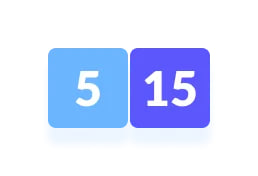
\includegraphics[scale=0.8]{Images/bi2.jpg}
        \end{figure}
        \subsection*{}
        As the order m = 3, so a node can have maximum $ m-1 = 2 $ keys. After inserting 25 the node has 3 keys. Now split the node and send the $\lceil \frac{m}{2}\rceil = 2$th element(i.e. key 15)  to the parents. And then attach the left half of the split node as left pointer of the parent node and right half as right pointer. Keep in mind to assign pointers if not already assigned.
        \begin{center}
            \color{red}\textbf{Insert 25}  
        \end{center}
        \begin{table}[ht]
            \centering
            \begin{tabular}{c c}
                    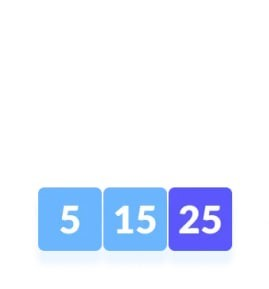
\includegraphics[scale=0.9]{Images/bi3_1_1.jpg} &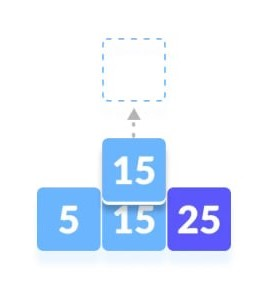
\includegraphics[scale=0.9]{Images/bi3_1_2.jpg}\\
                ({\color{red}i}) &({\color{red}ii}) \\
                    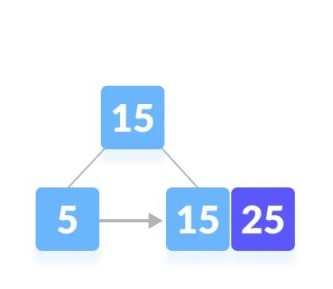
\includegraphics[scale=0.9]{Images/bi3_2_2.jpg} &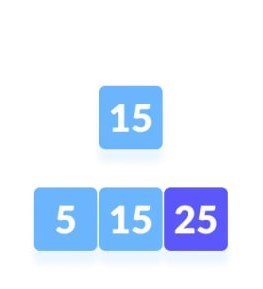
\includegraphics[scale=0.9]{Images/bi3_2_1.jpg}\\
                ({\color{red}iv}) &({\color{red}iii}) \\
            \end{tabular}
        \end{table} 
        \pagebreak
        \subsection*{}
        Now we are going to insert 35 into the B + tree. At first we need to find out the position at leaf level where the new key need to be inserted. As 35 is greater than 15 we need to go to the right child of the root node. We would go left if smaller. And we will follow the process until we are at any leaf node. 
        \begin{center}
            \color{red}\textbf{Insert 35}  
        \end{center}
        \begin{table}[ht]
            \centering
            \begin{tabular}{c c}
                    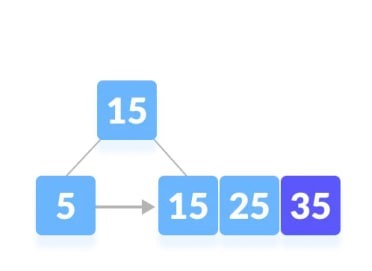
\includegraphics[scale=0.9]{Images/bi4_1_1.jpg} &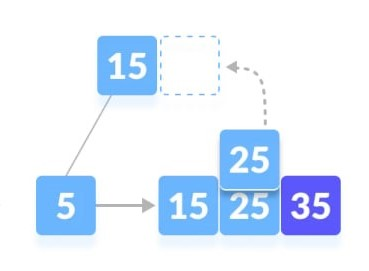
\includegraphics[scale=0.9]{Images/bi4_1_2.jpg}\\
                ({\color{red}i}) &({\color{red}ii}) \\
                    \multicolumn{2}{c}{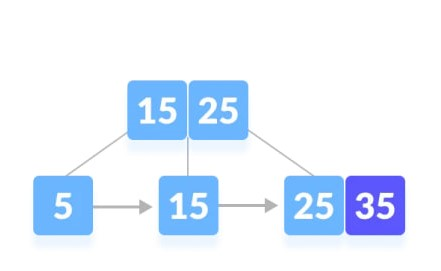
\includegraphics[scale=0.9]{Images/bi4_2.jpg}}\\
                \multicolumn{2}{c}{({\color{red}iii})}\\
            \end{tabular}
        \end{table}
        \subsection*{}
        Here we need to apply the 2nd case. After inserting 45 the leaf node is overflowing then we split the node as previous and send 35 to the parent node but the parent node already has 2 keys so it's also going to overflow. And we need to split this node also and then send 25 to the parent of the current node and assign it's left(if not already assigned) and right pointers. 
        \begin{center}
            \color{red}\textbf{Insert 45}  
        \end{center}
        \begin{table}[ht]
            \centering
            \begin{tabular}{c c}
                    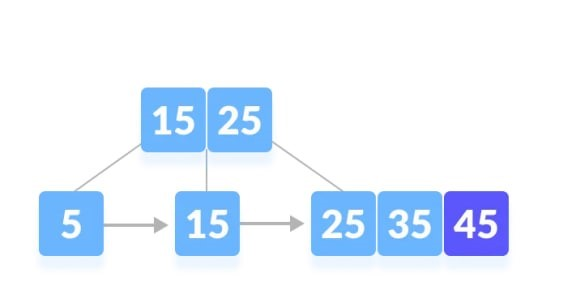
\includegraphics[scale=0.7]{Images/bi5_1_1.jpg} &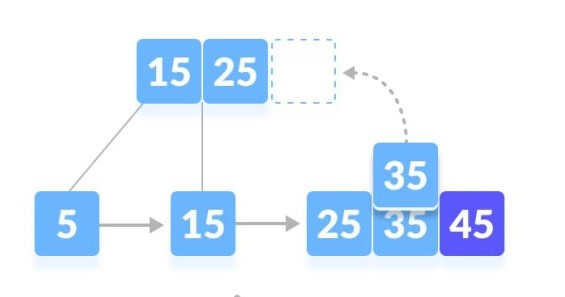
\includegraphics[scale=0.7]{Images/bi5_1_2.jpg}\\
                ({\color{red}i}) &({\color{red}ii}) \\
            \end{tabular}
        \end{table}
        \begin{center}
        \pagebreak    
        \end{center}
        \begin{table}[ht]
            \centering
            \begin{tabular}{c c}
                    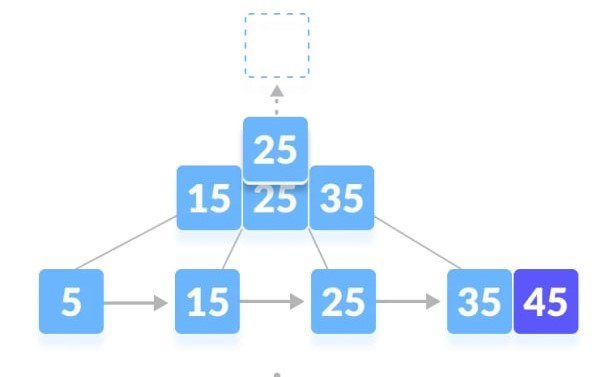
\includegraphics[scale=0.7]{Images/bi5_2_2.jpg} &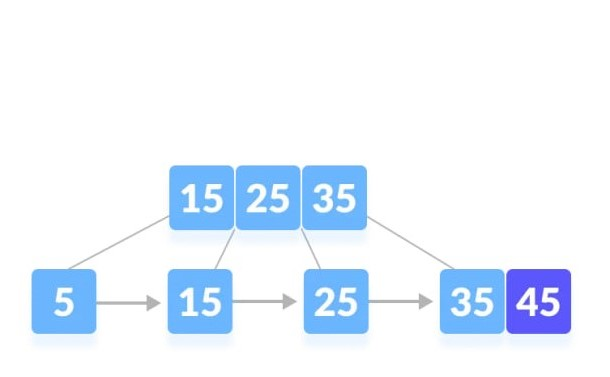
\includegraphics[scale=0.7]{Images/bi5_2_1.jpg}\\
                ({\color{red}iv}) &({\color{red}iii}) \\
                    \multicolumn{2}{c}{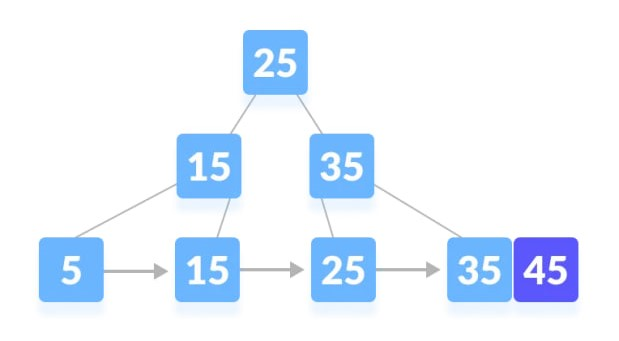
\includegraphics[scale=0.7]{Images/bi5_3.jpg}}\\
                \multicolumn{2}{c}{({\color{red}v})}\\
            \end{tabular}
        \end{table}  
 
    \subsection{Deletion from B+ Tree}
    Deleting an element in a B + tree consists of three main events: \begin{itemize}
        \item Searching the node where the key to be deleted exists.
        \item Deleting the key.
        \item Balancing the tree if required.
    \end{itemize}
   Underflow is a situation when there is less number of keys in a node than the minimum number of keys it should hold.\\
    Before going through the steps below, one must know these facts about a B+ tree of degree m. A node can have-
    \begin{enumerate}
        \item a maximum of m children. (i.e. 3)
        \item a maximum of m - 1 keys. (i.e. 2)
        \item a minimum of $\lceil m/2 \rceil$ children. (i.e. 2)
        \item a minimum of $\lceil m/2 \rceil - 1$ keys (except root node). (i.e., 1) \end{enumerate} 
    While deleting a key, we have to take care of the keys present in the internal nodes (i.e., indexes) as well because the values are redundant in a B+ tree. Search for the key to be deleted and then follow the following steps-
    \begin{itemize}
        \item \textbf{Case I:} The key to be deleted is present only at the leaf node not in the indexes (or internal nodes). There are two cases for it:
        \begin{enumerate}
            \item There is more than the minimum number of keys in the node. Simply delete the key.
            \begin{center}
                 \color{red}\textbf{Delete 40}
            \end{center}
            \begin{figure}
                \centering 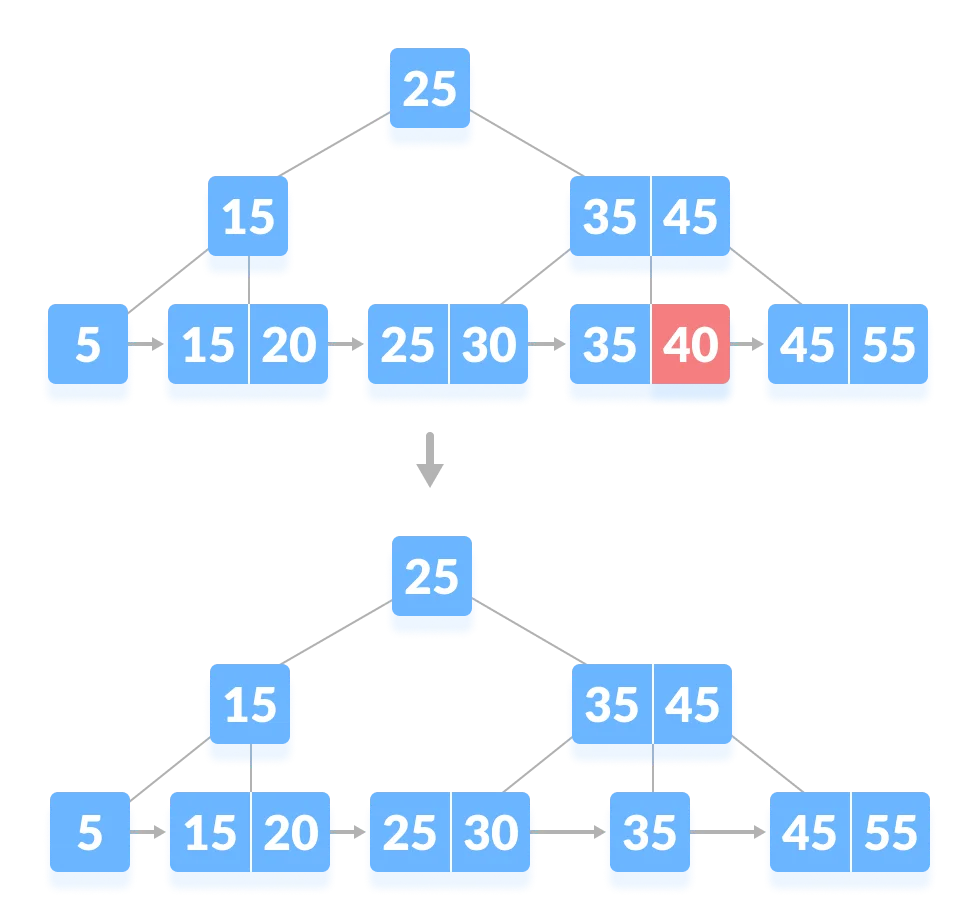
\includegraphics[scale = 0.3]{Images/deletion-1.png}
            \end{figure}
                   
            \item There is an exact minimum number of keys in the node. Delete the key and borrow a key from the immediate sibling. Add the median key of the sibling node to the parent.Deleting 5 from the tree below leads to this condition.\\
            \begin{center}
                 \color{red}\textbf{Delete 5}
            \end{center}
            \centering
            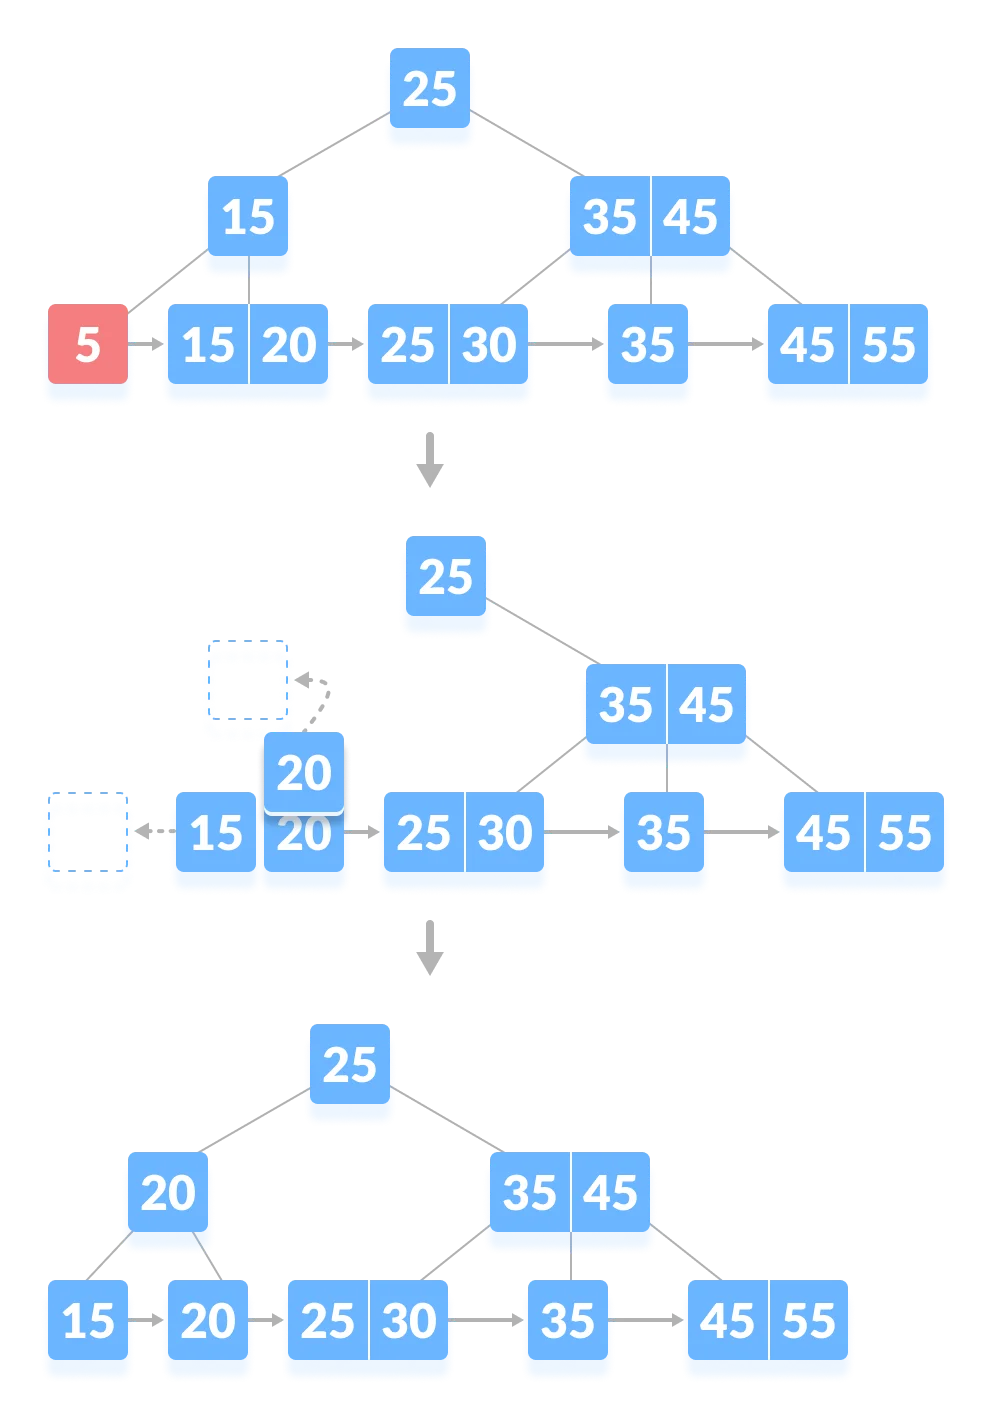
\includegraphics[scale = 0.3]{Images/deletion-2-btree.png}
        \end{enumerate}
    \end{itemize}
    \newpage
    \begin{itemize}
        \item \textbf{Case II:} The key to be deleted is present in the internal nodes as well. Then we have to remove them from the internal nodes as well. There are the following cases for this situation.
        \begin{enumerate}
            \item If there is more than the minimum number of keys in the node, simply delete the key from the leaf node and delete the key from the internal node as well. Fill the empty space in the internal node with the inorder successor.Deleting 45 from the tree below leads to this condition.\\
            \begin{center}
                 \color{red}\textbf{Delete 45}
            \end{center}
            \begin{figure}[ht]
                \centering
                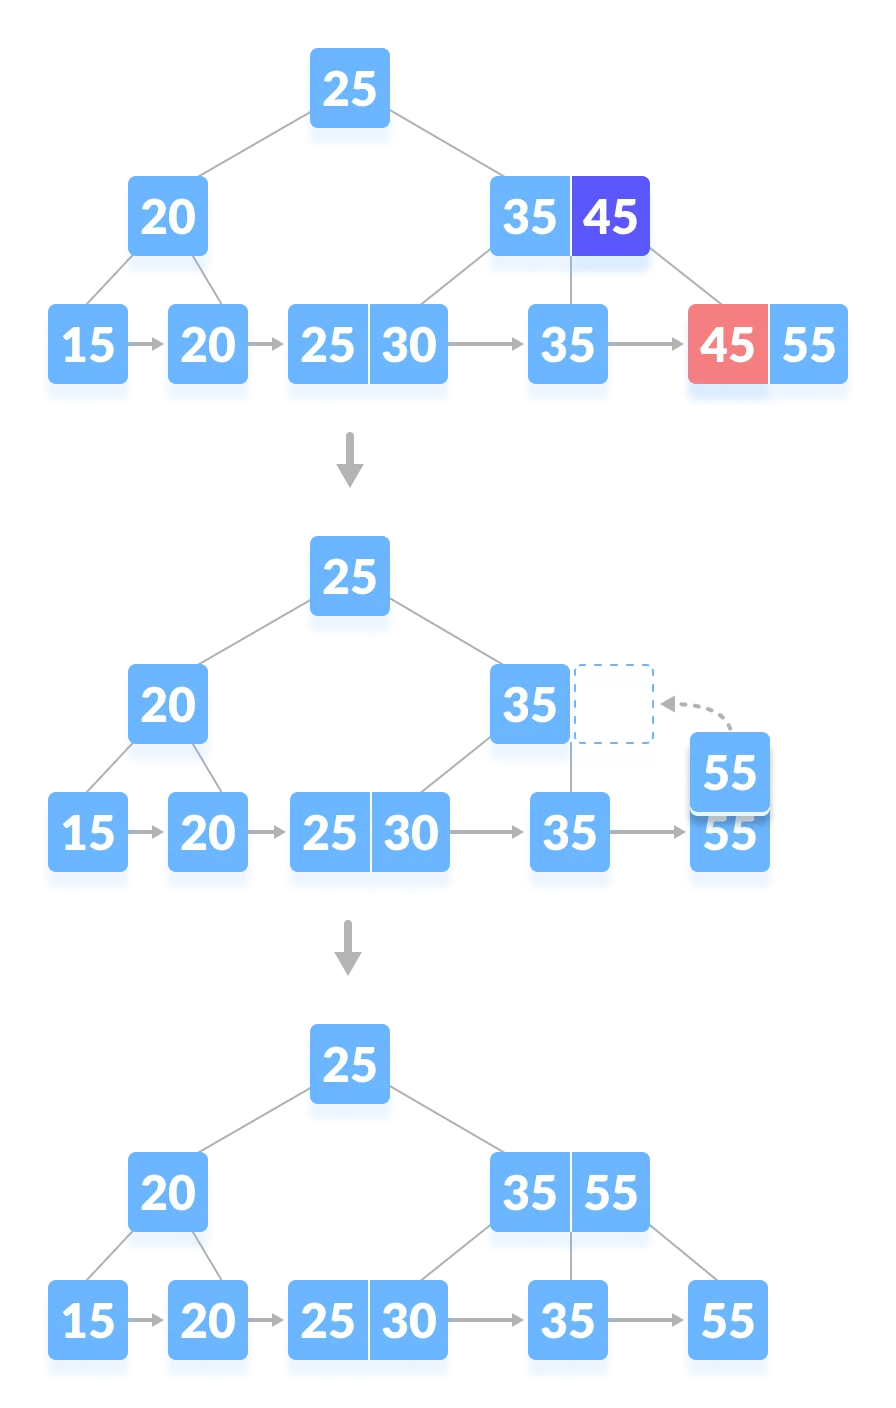
\includegraphics[scale = 0.4]{Images/deletion-3.png}
            \end{figure}
            \newpage
            \item If there is an exact minimum number of keys in the node, then delete the key and borrow a key from its immediate sibling (through the parent).Fill the empty space created in the index (internal node) with the borrowed key. Deleting 35 from the tree below leads to this condition.\\ 
            \begin{center}
                 \color{red}\textbf{Delete 35}
            \end{center}
            \begin{figure}[ht]
                \centering 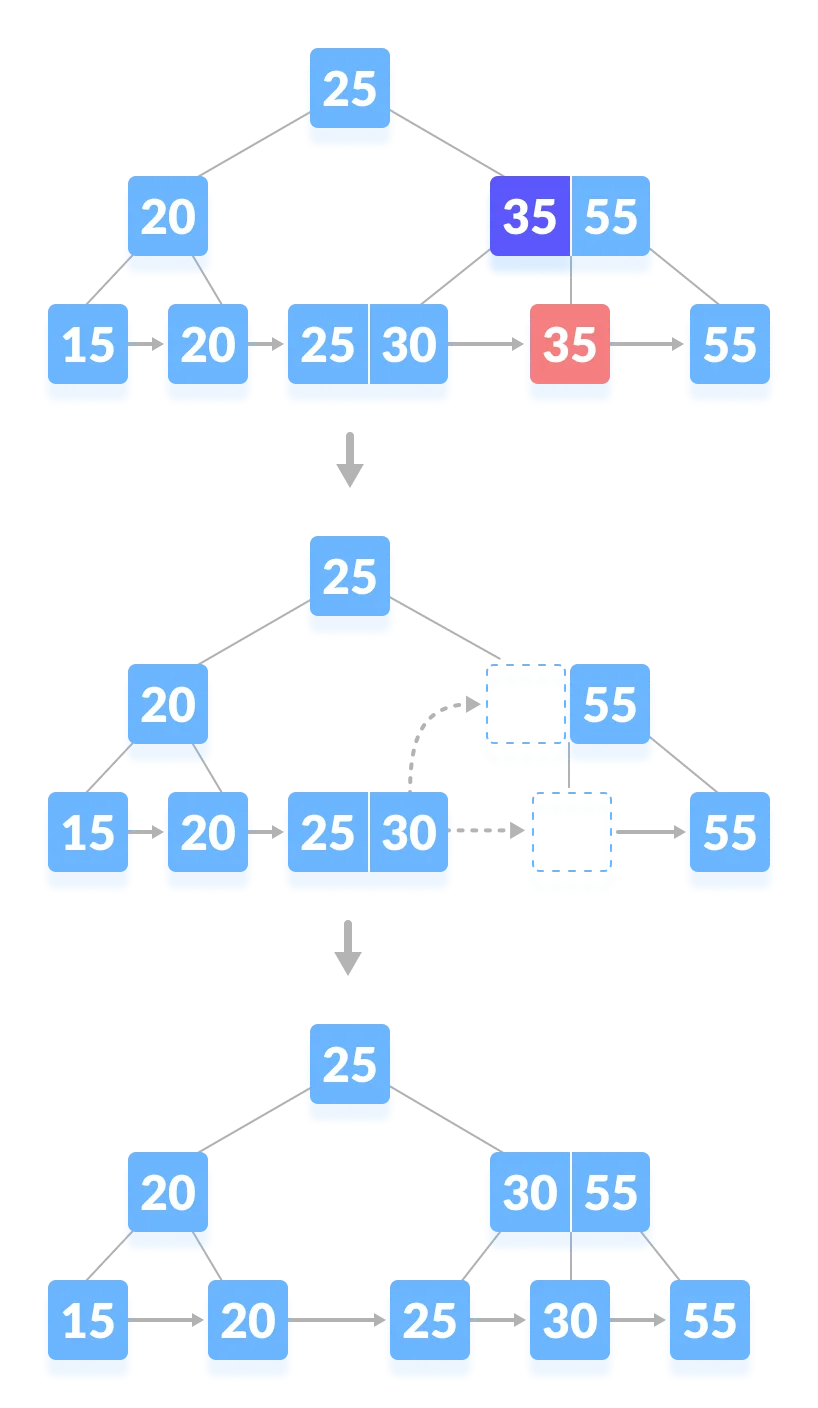
\includegraphics[scale = 0.4]{Images/deletion-4.png}
            \end{figure}
            
            \newpage
            \item This case is similar to Case II(1) but here, empty space is generated above the immediate parent node.After deleting the key, merge the empty space with its sibling.Fill the empty space in the grandparent node with the inorder successor. Deleting 25 from the tree below leads to this condition. \\
            \begin{center}
                 \color{red}\textbf{Delete 25}
            \end{center}
            \centering 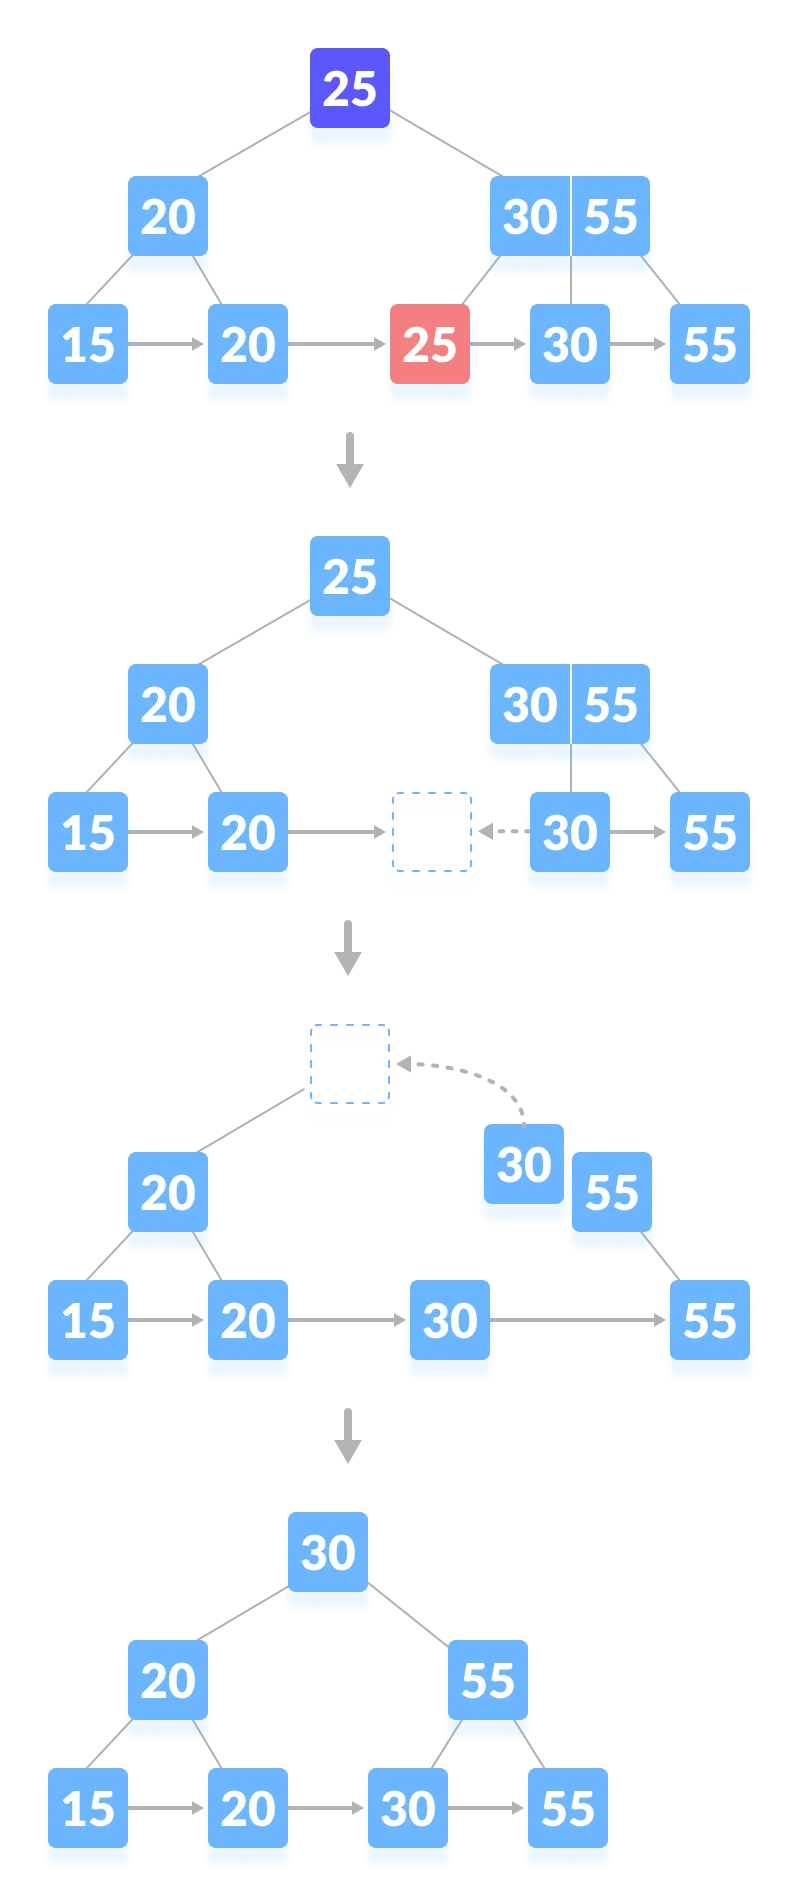
\includegraphics[scale = 0.4]{Images/deletion-5.png}
        \end{enumerate}
    \end{itemize}
    \newpage
    \begin{itemize}
            \item \textbf{Case III:} In this case, the height of the tree gets shrinked. It is a little complicated.Deleting 55 from the tree below leads to this condition. It can be understood in the illustrations below.
            \centering 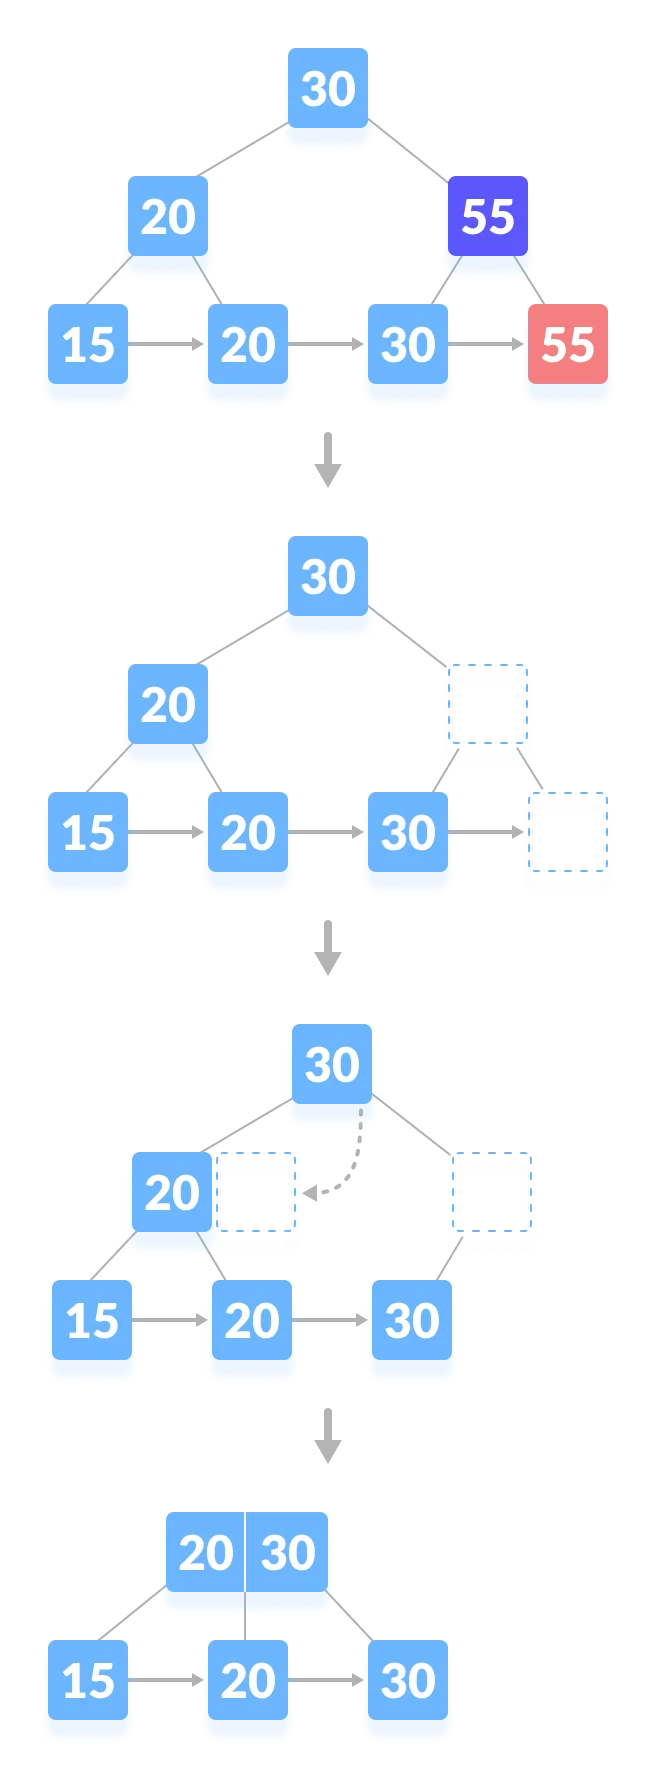
\includegraphics[scale = 0.4]{Images/deletion-6.png}
    \end{itemize}
    Pictures for simulating insertion and deletion are taken from \href{https://www.programiz.com/dsa/}{www.programiz.com}
    \subsection{Searching a key}
    When searching for a value \( k \) in a B+ tree, we start from the root and traverse down to find the leaf node that may contain the value \( k \). At each internal node, we select the appropriate child node to follow.\\ 

   An internal B+ tree node has at most \( b \leq m \) children, where each child represents a different sub-interval. We choose the corresponding child via a linear search of the \( b \) entries. When we reach a leaf node, we perform a linear search of its \( n \) elements for the desired key.\\
 
   Since we only traverse one branch of all the children at each level of the tree, we achieve a runtime of \( O(\log N) \), where \( N \) is the total number of keys stored in the leaves of the B+ tree.\\ \\ \\
    \textbf{Function Description:} Searches for a key \( k \) in the B+ tree starting from the root node \( \text{root} \).

    \begin{verbatim}
    function search(k, root) is
        let leaf = leaf_search(k, root)
        for leaf_key in leaf.keys() do
            if k = leaf_key then
                return true
        return false
    \end{verbatim}
    \textbf{Function Description:} Searches for a key \( k \) in the B+ tree starting from the node \( \text{node} \) and returns the leaf node where the key is located.

    \begin{verbatim}
    function leaf_search(k, node) is
        if node is a leaf then
            return node
        let p = node.children()
        let l = node.left_sided_intervals()
        assert |p| = |l| + 1
        let b = p.len()
        for i from 1 to m - 1 do
            if k <= l[i] then
                return leaf_search(k, p[i])
        return leaf_search(k, p[b])
    \end{verbatim}

\section{Time Complexity of B+ Tree Operations}
Consider a B+ tree having :
\begin{itemize}
    \item m : Order of the B+ tree.
    \item n: Total number of elements (or keys) stored in the B+ tree.
\end{itemize}
\begin{table}[ht]
        \centering
        \small % adjust font size
        \setlength{\tabcolsep}{10pt} % adjust column spacing
        \renewcommand{\arraystretch}{1.5} % adjust row spacing
        \begin{tabular}{|c|c|}
            \hline
            \textbf{B+ Tree Operation} & \textbf{Time Complexity}  \\
            \hline
            {Insertion} & {$O(\log_m n)$}\\
            \hline
            {Deletion} & {$O(\log_m n)$}\\
            \hline
            {Search} & {$O(\log_m n)$}\\
            \hline
        \end{tabular}
        \caption{Time Complexity}
    \end{table}
\begin{enumerate}
    \item \textbf{Search Operation (Find):}
    \begin{itemize}
        \item \textbf{Time Complexity:} \(O(\log_{m}^{n})\)
        \item \textbf{Explanation:} Searching in a B+ tree involves traversing from the root to the leaf level, which takes \(O(\log_{m}^{n})\) time, where \(n\) is the number of elements in the tree and \(m\) is the order of the tree. Since B+ trees are balanced, the height of the tree is logarithmic with respect to the number of elements and the order of the tree.
    \end{itemize}
    
    \item \textbf{Insertion Operation:}
    \begin{itemize}
        \item \textbf{Time Complexity:} \(O(\log_{m}^{n})\)
        \item \textbf{Explanation:} Inserting a new element into a B+ tree involves searching for the correct position to insert the element (\(O(\log_{m}^{n})\)) and potentially splitting nodes along the path to maintain the B+ tree properties. Splitting nodes may propagate up to the root, but the overall complexity remains \(O(\log_{m}^{n})\).
    \end{itemize}
    
    \item \textbf{Deletion Operation:}
    \begin{itemize}
        \item \textbf{Time Complexity:} \(O(\log_{m}^{n})\)
        \item \textbf{Explanation:} Deleting an element from a B+ tree also involves searching for the element to delete (\(O(\log_{m}^{n})\)) and potentially merging or redistributing nodes to maintain the B+ tree properties. Similar to insertion, the overall complexity remains \(O(\log_{m}^{n})\).
    \end{itemize}
    
    \item \textbf{Range Query Operation:}
    \begin{itemize}
        \item \textbf{Time Complexity:} \(O(\log_{m}^{n} + k)\)
        \item \textbf{Explanation:} Retrieving elements within a given range involves searching for the starting and ending points of the range (\(O(\log_{m}^{n})\)) and traversing leaf nodes to collect elements falling within the range (\(O(k)\), where \(k\) is the number of elements in the range).
    \end{itemize}
    
    \item \textbf{Splitting and Merging:}
    \begin{itemize}
        \item \textbf{Time Complexity:} \(O(1)\)
        \item \textbf{Explanation:} When splitting or merging nodes during insertion or deletion, the time complexity is constant per operation. However, these operations might propagate upwards, potentially affecting the entire height of the tree, but this is considered amortized constant time per operation.
    \end{itemize}
\end{enumerate}
\section{Advantages of B+ Trees}

\begin{itemize}
  \item \textbf{Efficient Search and Range Queries:} B+ trees provide efficient search operations and are optimized for range queries. They maintain data in sorted order, enabling logarithmic time complexity for search operations and efficient retrieval of ranges of data \cite{comer1979ubiquitous}.
\end{itemize}

\begin{itemize}
    \item \textbf{Concurrency Control and Performance} 
    B+ trees support efficient concurrency control mechanisms, making them suitable for concurrent database systems. They offer predictable performance characteristics and ensure consistency and isolation among concurrent transactions. If we use LOCKING for concurrency control, we need to update a single node at the same time, which can be done using B+ Tree very efficiently. If we use MULTI VERSION CONCURRENCY CONTROL(MVCC) , we have to update multiple nodes at the same time. It can be done using the persistence nature of B+ Tree. B+ Tree can be used as a persistent data structure that can remember its previous versions efficiently. We will only need to create logn more nodes every time that will be updated. \cite{agrawal1987concurrency}.
\end{itemize}
\begin{itemize}
  \item \textbf{Optimal Disk Access and Cache Efficiency:} B+ trees are designed to optimize disk I/O operations and maximize cache efficiency. They utilize node-based structures and node sizes that align well with the block size of storage devices, minimizing disk access and maximizing cache hits. \cite{oneil1992modern}.
\end{itemize}

\begin{itemize}
  \item \textbf{Support for Large Datasets:} B+ trees are suitable for managing large datasets efficiently. They can handle a large number of keys while maintaining logarithmic search and update times.For instance, if the number of data n = $10^6$ and order of tree is 100 then the height of the tree will be only 3. As a result , all the operations will be immensely fast. \cite{oneil1992modern}.
\end{itemize}

\begin{itemize}
  \item \textbf{Ordered Structure for Sequential Access:} B+ trees maintain data in sorted order, facilitating efficient sequential access to keys. This property simplifies operations such as range scans and sequential processing of data \cite{garcia2000database}.
\end{itemize}

\begin{itemize}
  \item \textbf{Balanced Tree:} B+ trees are balanced trees, ensuring that the height of the tree remains minimal. This balance ensures that operations such as insertion, deletion, and search have consistent performance characteristics \cite{bayer1972design}.
\end{itemize}

\section{Real Life Application of B+ Tree}
    \begin{itemize}
        \item \textbf{Database Indexing:}\\B+ trees are widely used in database management systems for indexing. They enable effective retrieval of data based on indexed characteristics, resulting in faster query execution times. For example, in a customer database, a B+ tree index on the "customerId" property may be used to quickly retrieve customer records by ID.
    \end{itemize}

    \begin{itemize}
        \item \textbf{File Systems:}\\In file systems, B+ trees are used to manage and organize file information and directory hierarchies. They make it easier to store and retrieve file metadata, including size, creation date, and rights, and speed up file path lookup. For example, B+ trees are used for directory indexing in the Ext4 file system, which is widely found in Linux versions.
    \end{itemize}

    \begin{itemize}
        \item \textbf{Distributed Databases:}\\In distributed databases, where data is spread across multiple nodes, B+ trees are employed for maintaining distributed indexes. These indexes allow for efficient query processing and data retrieval across distributed nodes while ensuring data consistency and fault tolerance.
    \end{itemize}

    \begin{itemize}
        \item \textbf{Geo-spatial Databases:}\\B+ trees are well-suited for indexing Geo-spatial data such as coordinates, shapes, and spatial relationships. They enable efficient spatial queries such as range searches, nearest-neighbor searches, and spatial joins. Geo-spatial databases, used in applications such as Geographic Information Systems (GIS) and location-based services, often utilize B+ trees for spatial indexing.
    \end{itemize}

    \begin{itemize}
        \item \textbf{File Sharing Networks:}\\B+ trees can be utilized in peer-to-peer file sharing networks for maintaining distributed indexes of available files. They facilitate efficient lookup and retrieval of files based on various attributes such as file name, size, and type, thereby enhancing the overall performance of the file sharing network.
    \end{itemize}



    \begin{itemize}
        \item \textbf{Web Browsers:}\\B+ trees are employed in web browsers for managing bookmarks and history data. They enable quick retrieval of URLs based on search queries and facilitate efficient storage and retrieval of browsing history, thereby enhancing the browsing experience for users.
    \end{itemize}
    \section{A Sample Implementation of B+ Tree Using Python} 
    \lstinputlisting[language=Python]{bplustree.py}
    Find the code \href{https://www.programiz.com/dsa/deletion-from-a-b-plus-tree}{here}\\ \\
    \section{Discussion}
    Initially, grasping the concept of B+ trees seemed daunting due to their complex structure and operations. However, as we delved deeper into the topic, we gradually gained clarity and appreciation for their design principles.\\ \\
    Engaging in hands-on practice, including implementing B+ trees from scratch and working on practical exercises, significantly enhanced our understanding. It allowed us to visualize the inner workings of B+ trees and appreciate their efficiency in real-world scenarios.\\ \\
    While learning about B+ trees, we encountered challenges in understanding certain aspects such as node splitting, merging, and balancing. However, with perseverance and guidance, we overcame these challenges and strengthened our grasp of the concepts. Collaborating with peers and discussing concepts, challenges, and solutions greatly enriched our learning experience. Sharing insights, exploring different perspectives, and collaborating on the presentation fostered a supportive learning environment.\\ \\
    Learning about B+ trees has not only expanded our technical knowledge, but also sharpened our problem-solving and critical thinking skills. It has equipped us with a powerful tool for efficiently managing and accessing large datasets in diverse applications.
\pagebreak
\bibliographystyle{plain}
\bibliography{References}
    
\end{document}